\documentclass[tikz]{standalone}

% tikz
\usepackage{tikz, pgfplots}
% i wish external worked but idk it sucks
%\usetikzlibrary{external}
%\tikzexternalize[prefix=figures/]

% for function graph
\usetikzlibrary{positioning}
\usetikzlibrary{shapes.geometric}
\usetikzlibrary{positioning}
\usetikzlibrary{shapes.misc}
\tikzset{
dot/.style = {circle, fill=#1, minimum size=5pt,
              inner sep=0pt, outer sep=0pt},
dot/.default = black % size of the circle diameter
}
\tikzset{cross/.style={cross out, draw=black, minimum size=2*(#1-\pgflinewidth), inner sep=0pt, outer sep=0pt},
%default radius will be 1pt. 
cross/.default={1pt}}

 % for braces
\usetikzlibrary{decorations.pathreplacing}
% for hashing area
\usetikzlibrary{patterns}
% tableaux var, signe
% source https://www.sqlpac.com/fr/documents/latex-package-tkz-tab-tikz-tableaux-de-signes-et-de-variations-de-fonctions.html
\usepackage{tkz-tab}
%%%%%%%%%%%%%%%%%%%%%%%%%%%%%%
% SELF MADE COLORS
%%%%%%%%%%%%%%%%%%%%%%%%%%%%%%


\definecolor{myg}{RGB}{56, 140, 70}
\definecolor{myb}{RGB}{45, 111, 177}
\definecolor{myr}{RGB}{199, 68, 64}
\definecolor{mytheorembg}{HTML}{F2F2F9}
\definecolor{mytheoremfr}{HTML}{00007B}
\definecolor{mylenmabg}{HTML}{FFFAF8}
\definecolor{mylenmafr}{HTML}{983b0f}
\definecolor{mypropbg}{HTML}{f2fbfc}
\definecolor{mypropfr}{HTML}{191971}
\definecolor{myexamplebg}{HTML}{F2FBF8}
\definecolor{myexamplefr}{HTML}{88D6D1}
\definecolor{myexampleti}{HTML}{2A7F7F}
\definecolor{mydefinitbg}{HTML}{E5E5FF}
\definecolor{mydefinitfr}{HTML}{3F3FA3}
\definecolor{notesgreen}{RGB}{0,162,0}
\definecolor{myp}{RGB}{197, 92, 212}
\definecolor{mygr}{HTML}{2C3338}
\definecolor{myred}{RGB}{127,0,0}
\definecolor{myyellow}{RGB}{169,121,69}
\definecolor{myexercisebg}{HTML}{F2FBF8}
\definecolor{myexercisefg}{HTML}{88D6D1}
\definecolor{doc}{RGB}{0,60,110}

% manim colors because they're beautiful
% https://docs.manim.community/en/stable/reference/manim.utils.color.manim_colors.html

\definecolor{BLACK}{HTML}{000000}\definecolor{BLUE}{HTML}{58C4DD}\definecolor{BLUE_A}{HTML}{C7E9F1}\definecolor{BLUE_B}{HTML}{9CDCEB}\definecolor{BLUE_C}{HTML}{58C4DD}\definecolor{BLUE_D}{HTML}{29ABCA}\definecolor{BLUE_E}{HTML}{236B8E}\definecolor{DARKER_GRAY}{HTML}{222222}\definecolor{DARKER_GREY}{HTML}{222222}\definecolor{DARK_BLUE}{HTML}{236B8E}\definecolor{DARK_BROWN}{HTML}{8B4513}\definecolor{DARK_GRAY}{HTML}{444444}\definecolor{DARK_GREY}{HTML}{444444}\definecolor{GOLD}{HTML}{F0AC5F}\definecolor{GOLD_A}{HTML}{F7C797}\definecolor{GOLD_B}{HTML}{F9B775}\definecolor{GOLD_C}{HTML}{F0AC5F}\definecolor{GOLD_D}{HTML}{E1A158}\definecolor{GOLD_E}{HTML}{C78D46}\definecolor{GRAY}{HTML}{888888}\definecolor{GRAY_A}{HTML}{DDDDDD}\definecolor{GRAY_B}{HTML}{BBBBBB}\definecolor{GRAY_BROWN}{HTML}{736357}\definecolor{GRAY_C}{HTML}{888888}\definecolor{GRAY_D}{HTML}{444444}\definecolor{GRAY_E}{HTML}{222222}\definecolor{GREEN}{HTML}{83C167}\definecolor{GREEN_A}{HTML}{C9E2AE}\definecolor{GREEN_B}{HTML}{A6CF8C}\definecolor{GREEN_C}{HTML}{83C167}\definecolor{GREEN_D}{HTML}{77B05D}\definecolor{GREEN_E}{HTML}{699C52}\definecolor{GREY}{HTML}{888888}\definecolor{GREY_A}{HTML}{DDDDDD}\definecolor{GREY_B}{HTML}{BBBBBB}\definecolor{GREY_BROWN}{HTML}{736357}\definecolor{GREY_C}{HTML}{888888}\definecolor{GREY_D}{HTML}{444444}\definecolor{GREY_E}{HTML}{222222}\definecolor{LIGHTER_GRAY}{HTML}{DDDDDD}\definecolor{LIGHTER_GREY}{HTML}{DDDDDD}\definecolor{LIGHT_BROWN}{HTML}{CD853F}\definecolor{LIGHT_GRAY}{HTML}{BBBBBB}\definecolor{LIGHT_GREY}{HTML}{BBBBBB}\definecolor{LIGHT_PINK}{HTML}{DC75CD}\definecolor{LOGO_BLACK}{HTML}{343434}\definecolor{LOGO_BLUE}{HTML}{525893}\definecolor{LOGO_GREEN}{HTML}{87C2A5}\definecolor{LOGO_RED}{HTML}{E07A5F}\definecolor{LOGO_WHITE}{HTML}{ECE7E2}\definecolor{MAROON}{HTML}{C55F73}\definecolor{MAROON_A}{HTML}{ECABC1}\definecolor{MAROON_B}{HTML}{EC92AB}\definecolor{MAROON_C}{HTML}{C55F73}\definecolor{MAROON_D}{HTML}{A24D61}\definecolor{MAROON_E}{HTML}{94424F}\definecolor{ORANGE}{HTML}{FF862F}\definecolor{PINK}{HTML}{D147BD}\definecolor{PURE_BLUE}{HTML}{0000FF}\definecolor{PURE_GREEN}{HTML}{00FF00}\definecolor{PURE_RED}{HTML}{FF0000}\definecolor{PURPLE}{HTML}{9A72AC}\definecolor{PURPLE_A}{HTML}{CAA3E8}\definecolor{PURPLE_B}{HTML}{B189C6}\definecolor{PURPLE_C}{HTML}{9A72AC}\definecolor{PURPLE_D}{HTML}{715582}\definecolor{PURPLE_E}{HTML}{644172}\definecolor{RED}{HTML}{FC6255}\definecolor{RED_A}{HTML}{F7A1A3}\definecolor{RED_B}{HTML}{FF8080}\definecolor{RED_C}{HTML}{FC6255}\definecolor{RED_D}{HTML}{E65A4C}\definecolor{RED_E}{HTML}{CF5044}\definecolor{TEAL}{HTML}{5CD0B3}\definecolor{TEAL_A}{HTML}{ACEAD7}\definecolor{TEAL_B}{HTML}{76DDC0}\definecolor{TEAL_C}{HTML}{5CD0B3}\definecolor{TEAL_D}{HTML}{55C1A7}\definecolor{TEAL_E}{HTML}{49A88F}\definecolor{WHITE}{HTML}{FFFFFF}\definecolor{YELLOW}{HTML}{FFFF00}\definecolor{YELLOW_A}{HTML}{FFF1B6}\definecolor{YELLOW_B}{HTML}{FFEA94}\definecolor{YELLOW_C}{HTML}{FFFF00}\definecolor{YELLOW_D}{HTML}{F4D345}\definecolor{YELLOW_E}{HTML}{E8C11C}

% Schwartz
\renewcommand{\S}{\mathcal{S}} % \S est le signe paragraphe normalement

% corps
\newcommand{\C}{\mathcal{C}}
\newcommand{\R}{\mathbb{R}}
\newcommand{\Rnn}{\mathbb{R}^{2n}}
\newcommand{\Z}{\mathbb{Z}}
\newcommand{\N}{\mathbb{N}}
\newcommand{\Q}{\mathbb{Q}}

% domain
\newcommand{\D}{\mathcal{D}}

% order notations
\renewcommand{\O}{\mathcal{O}}

% japanese bracket
\newcommand{\japb}[1]{\langle #1 \rangle}

% arrows over partial derivatives
\newcommand{\lp}{\overleftarrow{\partial}}
\newcommand{\rp}{\overrightarrow{\partial}}

% quantization
\newcommand{\h}{\hbar}
\newcommand{\Opht}{\textrm{Op}_{\h}^{t}}
\newcommand{\Op}[2][\hbar]{\textrm{Op}_{#1}^{#2}}

% omega functions
\newcommand{\omegap}[2][\rho_0]{\omega(\partial_{#1},\partial_{#2})}
\newcommand{\omegar}[2][\rho_0]{\omega(#1,#2)}
% PLUS INFTY AND MINUS INFTY WITH NO SPACE
\newcommand{\pinfty}{{+}\infty}
\newcommand{\minfty}{{-}\infty}

\begin{document}
%
	% page 1
	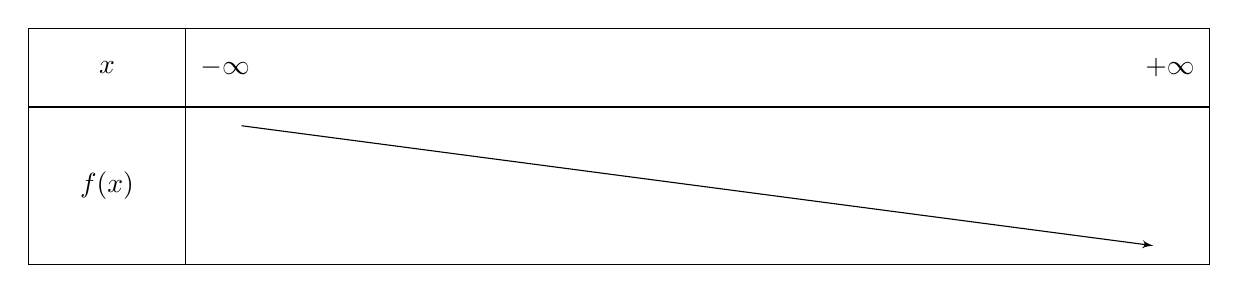
\begin{tikzpicture}
		\tkzTabInit
		 [espcl=4]
	       		{$x$ / 1 , $f(x)$ / 2}
	       		{$\minfty$,,, $\pinfty$}
	       		
		\tkzTabVar
			{+/, R/, R/, -/}
	\end{tikzpicture}
	% page 2
	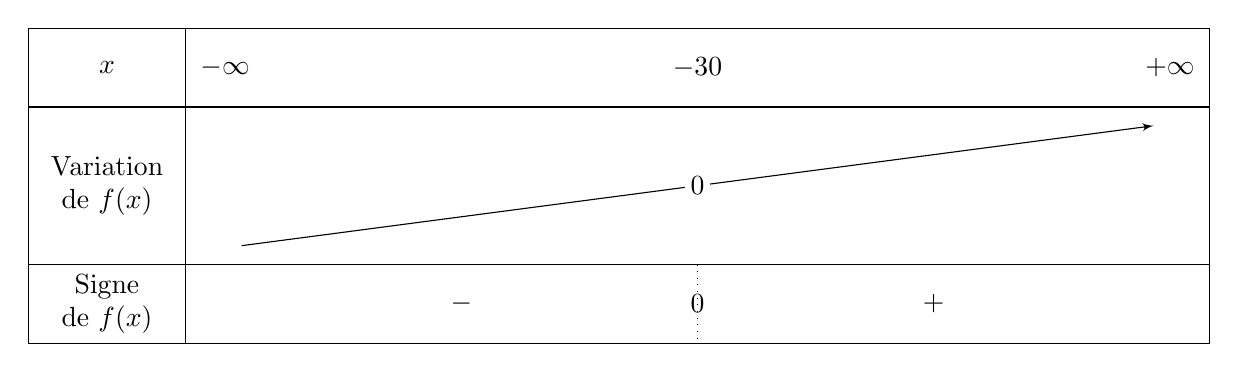
\begin{tikzpicture}
		\tkzTabInit
		 %[lgt=3,espcl=1.5]
	       		{$x$ / 1 , Variation de $f(x)$ / 2, Signe de $f(x)$ / 1}
	       		{$\minfty$,, $-30$,, $\pinfty$}
	       		
		\tkzTabVar
			{-/,  R/, R/, R/, +/}
		\tkzTabIma
			{1}{5}{3}{0}
			
		\tkzTabLine
			{,,-,,z,,+}
	\end{tikzpicture}
	% page 3
	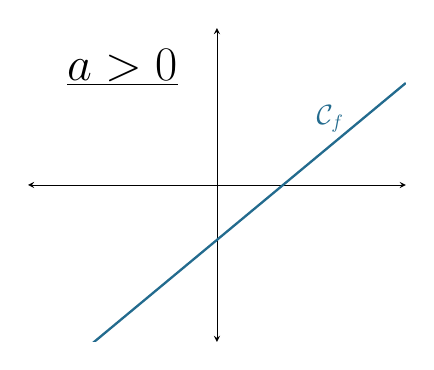
\begin{tikzpicture}[>=stealth, scale=.7]
	\begin{axis}[xmin = -1, xmax=1, ymin=-2, ymax=2, axis x line=middle, axis y line=middle, axis line style=<->, xlabel={}, ylabel={},ticks = none, grid=none]
	
		\addplot[very thick, BLUE_E, domain = -1:1] {2*x-.7} node[pos=.8, above=3pt] {\Large $\C_f$};
		\draw (axis cs: -.5, 1.5) node {\Huge \underline{$a>0$}};
	\end{axis}
	\end{tikzpicture}
	% page 4
	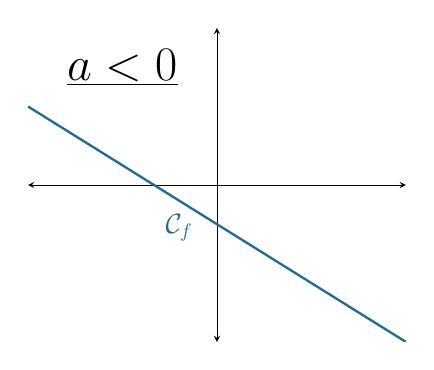
\begin{tikzpicture}[>=stealth, scale=.7]
	\begin{axis}[xmin = -1, xmax=1, ymin=-2, ymax=2, axis x line=middle, axis y line=middle, axis line style=<->, xlabel={}, ylabel={},ticks = none, grid=none]
	
		\addplot[very thick, BLUE_E, domain = -1:1] {-1.5*x-.5} node[pos=.4, below=3pt] {\Large $\C_f$};
		\draw (axis cs: -.5, 1.5) node {\Huge \underline{$a<0$}};
	\end{axis}
	\end{tikzpicture}
	% page 5
	\begin{tikzpicture}[>=stealth, scale=.7]
	\begin{axis}[xmin = -1, xmax=1, ymin=-2, ymax=2, axis x line=middle, axis y line=middle, axis line style=<->, xlabel={}, ylabel={},ticks = none, grid=none,]
	
		\addplot[very thick, BLUE_E, domain = -1:1] {-.6} node[pos=.7, below] {\Large $\C_f$};
		\draw (axis cs: -.5, 1.5) node {\Huge \underline{$a=0$}};
	\end{axis}
	\end{tikzpicture}
	% page 6
	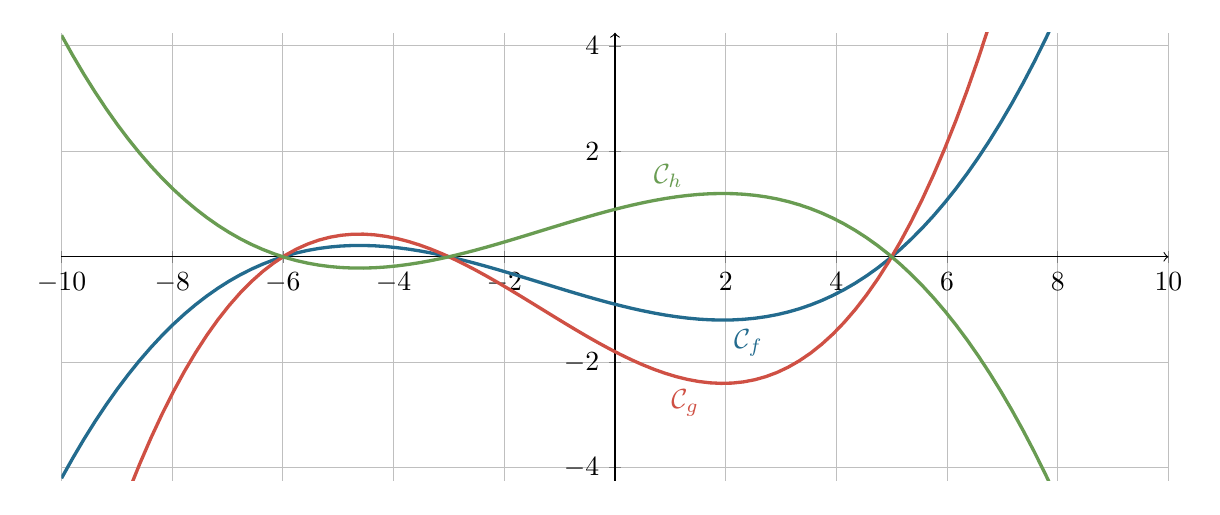
\begin{tikzpicture}[scale=1]
		\begin{axis}[xmin = -10, xmax=10, ymin=-4.25, ymax=4.25, axis x line=middle, axis y line=middle, axis line style=->, grid=both,
		x=20pt,
	    	]
		% g cos
		\addplot[no marks, BLUE_E, -, very thick] expression[domain=-10:10, samples=100]{.01*(x+6)*(x+3)*(x-5)}
		node[pos=.5, below]{$\mathcal{C}_f$};
		\addplot[no marks, RED_E, -, very thick] expression[domain=-10:10, samples=100]{.02*(x+6)*(x+3)*(x-5)}
		node[pos=.4, below]{$\mathcal{C}_g$};
		\addplot[no marks, GREEN_E, -, very thick] expression[domain=-10:10, samples=100]{-.01*(x+6)*(x+3)*(x-5)}
		node[pos=.45, above]{$\mathcal{C}_h$};
		\end{axis}
	\end{tikzpicture}
	% page 7
	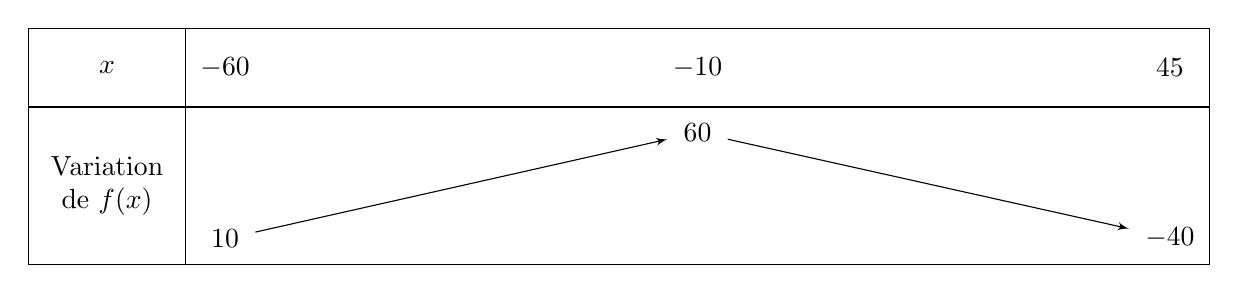
\begin{tikzpicture}
		\tkzTabInit
		 %[lgt=3,espcl=1.5]
	       		{$x$ / 1 , Variation de $f(x)$ / 2}
	       		{$-60$,, $-10$,, $45$}
	       		
		\tkzTabVar
			{-/$10$, R/, +/$60$, R/, -/$-40$}
	\end{tikzpicture}
	% page 8
	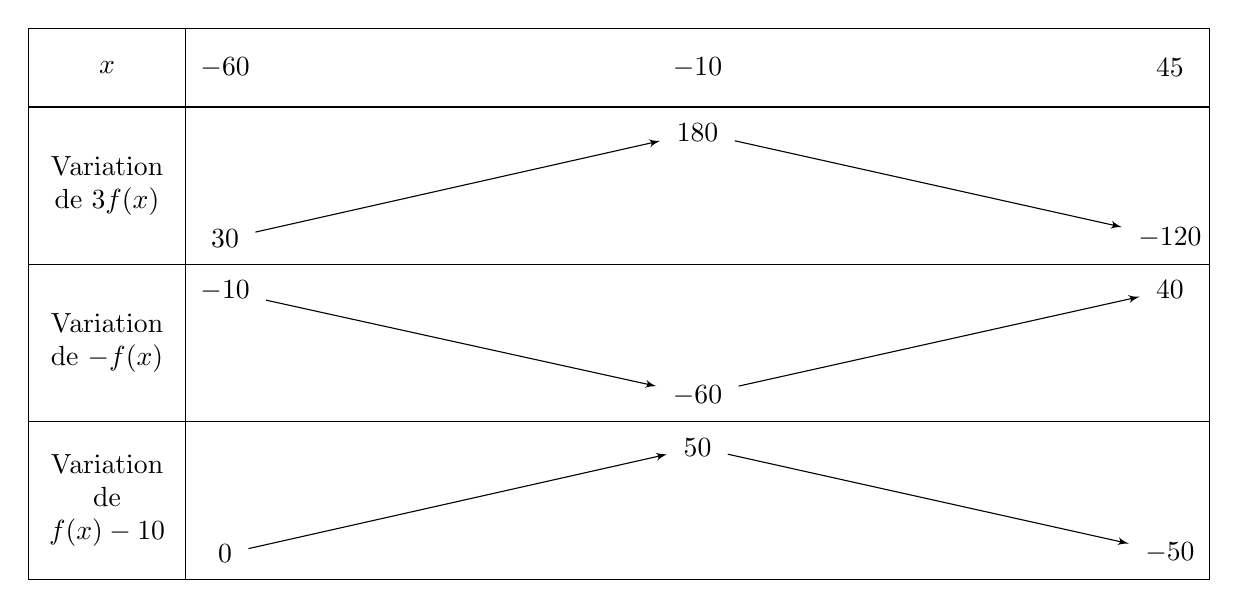
\begin{tikzpicture}
		\tkzTabInit
		 %[lgt=3,espcl=1.5]
	       		{$x$ / 1 , Variation de $3f(x)$ / 2, Variation de $-f(x)$ / 2, Variation de $f(x)-10$ / 2}
	       		{$-60$,, $-10$,, $45$}
	       		
		\tkzTabVar
			{-/$30$, R/, +/$180$, R/, -/$-120$}
		\tkzTabVar
			{+/$-10$, R/, -/$-60$, R/, +/$40$}
		\tkzTabVar
			{-/$0$, R/, +/$50$, R/, -/$-50$}
	\end{tikzpicture}
	
	% exe:var1
	% page 9
	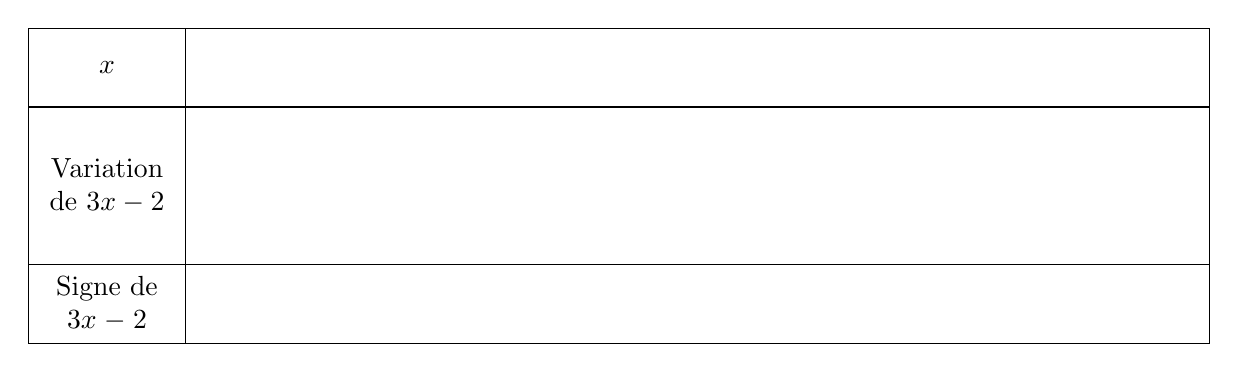
\begin{tikzpicture}
		\tkzTabInit
	       		{$x$ / 1 , Variation de $3x-2$ / 2, Signe de $3x-2$ / 1}
	       		{,,,,}
	\end{tikzpicture}
	
	% exe:var1
	% page 10
	\begin{tikzpicture}
		\tkzTabInit
	       		{$x$ / 1 , Variation de $3x-2$ / 2, Signe de $3x-2$ / 1}
	       		{  $-10$ ,,  $\dfrac23$ ,,  $12$ }
	       	
		\tkzTabVar
			{-/$-32$, R/, R/, R/, +/$34$}
		\tkzTabIma
			{1}{5}{3}{0}
		\tkzTabLine
			{,,-,,z,,+}
	\end{tikzpicture}
	
	% exe:var2
	% page 11
	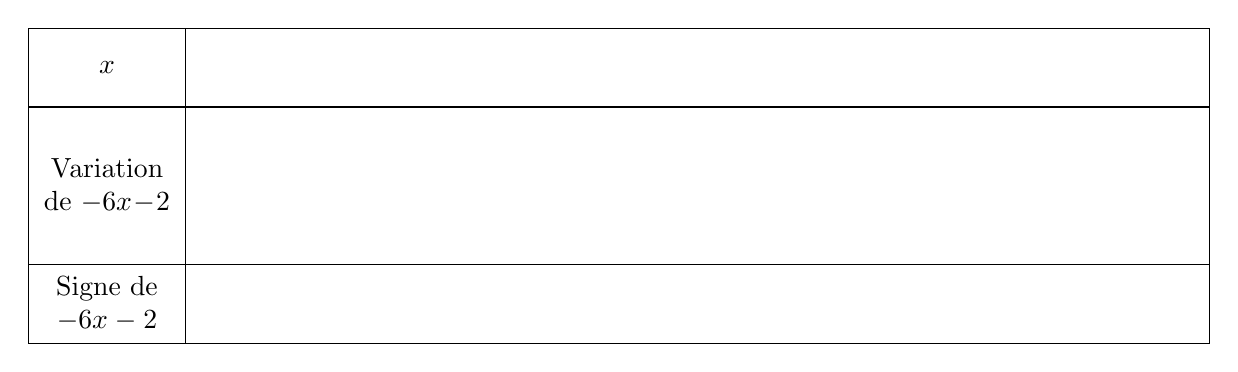
\begin{tikzpicture}
		\tkzTabInit
	       		{$x$ / 1 , Variation de $-6x-2$ / 2, Signe de $-6x-2$ / 1}
	       		{,,,,}
	\end{tikzpicture}
	
	% exe:var2
	% page 12
	\begin{tikzpicture}
		\tkzTabInit
	       		{$x$ / 1 , Variation de $-6x-2$ / 2, Signe de $-6x-2$ / 1}
	       		{  $-10$ ,,  $-\dfrac13$ ,,  $8$ }
	       	
		\tkzTabVar
			{+/$58$, R/, R/, R/, -/$-50$}
		\tkzTabIma
			{1}{5}{3}{0}
		\tkzTabLine
			{,,+,,z,,-}
	\end{tikzpicture}
	
	% exe:var3
	% page 13
	\begin{tikzpicture}
		\tkzTabInit
	       		{$x$ / 1 , Variation de $-3$ / 2, Signe de $-3$ / 1}
	       		{,,,,}
	\end{tikzpicture}
	
	% exe:var3
	% page 14
	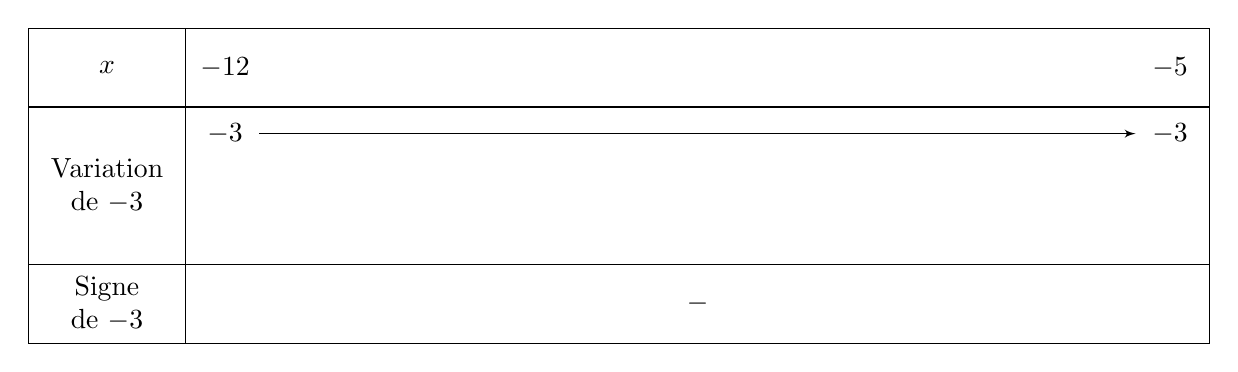
\begin{tikzpicture}
		\tkzTabInit
	       		{$x$ / 1 , Variation de $-3$ / 2, Signe de $-3$ / 1}
	       		{  $-12$ ,,,,  $-5$ }
		\tkzTabVar
			{+/$-3$, R/, R/, R/,+/$-3$}
		\tkzTabLine
			{,,,,-,,}
	\end{tikzpicture}
	
	% exe:var4
	% page 15
	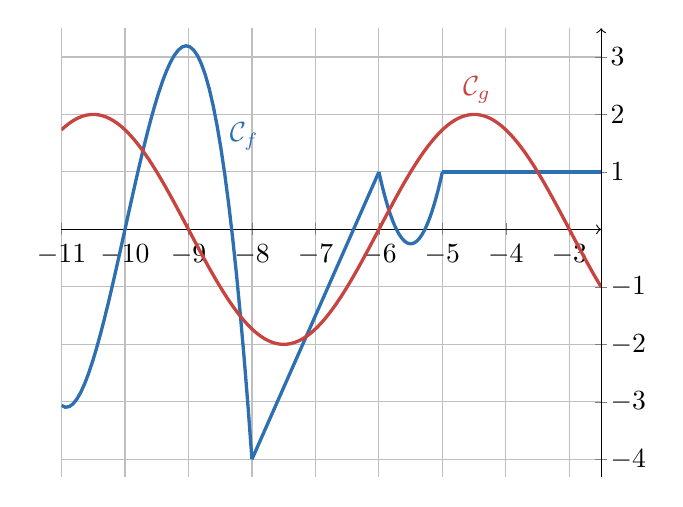
\begin{tikzpicture}[scale=1]
		\begin{axis}[xmin = -11, xmax=-2.5, ymin=-4.3, ymax=3.5, axis x line=middle, axis y line=middle, axis line style=->, grid=both, ytick={-4,-3,...,2,3}, xtick={-11, -10,...,-4,-3},
    every y tick label/.style={
        anchor=near yticklabel opposite,
        xshift=0.2em,
    }]
    			%f de l'éval f° affines
			\addplot[no marks, myb, -, very thick] expression[domain=-11:-8, samples=50]{5*(x+10)*(x^3 - 300*x - 1920)/80} 
			node[pos=.6, right]{$\mathcal{C}_f$};
			\addplot[no marks, myb, -, very thick] expression[domain=-8:-6, samples=2]{5*(x/2 + 3.2)};
			\addplot[no marks, myb, -, very thick] expression[domain=-6:-5, samples=50]{5*((x+5.5)^2 - 0.5^2 + 0.2)};
			\addplot[no marks, myb, -, very thick] expression[domain=-5:-2.5, samples=2]{5*0.2};
			
			% g sinus
			\addplot[no marks, myr, -, very thick] expression[domain=-11:-2.5, samples=500]{2*sin(x*60)}
			node[pos=.75, above]{$\mathcal{C}_g$};
		\end{axis}
	\end{tikzpicture}
	
	% exe:var4
	% pages 16-19
	\begin{tikzpicture}
		\tkzTabInit
		 [lgt=3,espcl=2]
	       		{$x$ / 1 , Variation de $f(x)$ / 2}
	       		{,,,,,,}
	       	
	\end{tikzpicture}
	\begin{tikzpicture}
		\tkzTabInit
		[lgt=3,espcl=3]
	       		{$x$ / 1 , Variation de $g(x)$ / 2}
	       		{,,,,}
	\end{tikzpicture}
	
	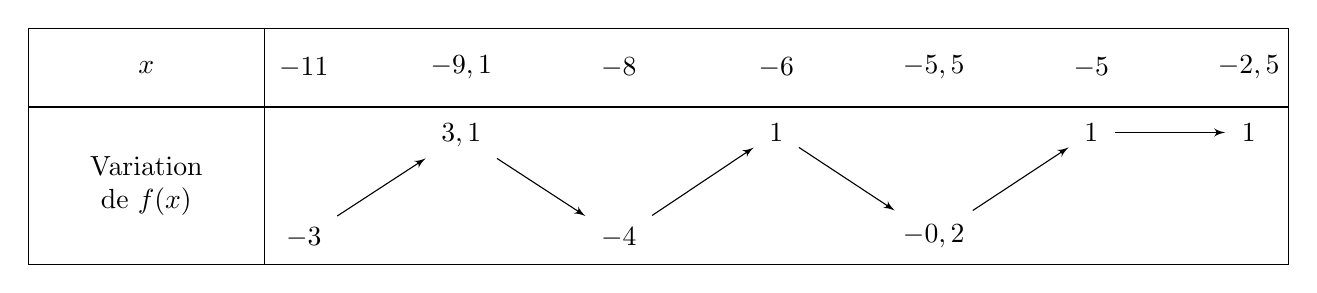
\begin{tikzpicture}
		\tkzTabInit
		 [lgt=3,espcl=2]
	       		{$x$ / 1 , Variation de $f(x)$ / 2}
	       		{ $-11$ , ${-9,1}$ , {$-8$} , {$-6$} ,  {$-5,5$} ,  {$-5$} ,  {$-2,5$} }
	       	
	       	
		\tkzTabVar
			{-/$-3$, +/${3,1}$, -/$-4$, +/$1$, -/${-0,2}$, +/$1$, +/$1$}
	\end{tikzpicture}
	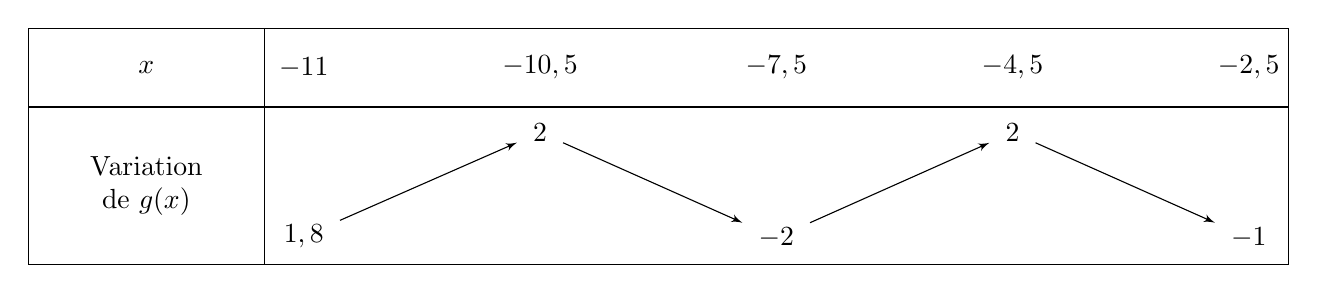
\begin{tikzpicture}
		\tkzTabInit
		[lgt=3,espcl=3]
	       		{$x$ / 1 , Variation de $g(x)$ / 2}
	       		{ $-11$ , ${-10,5}$ , {$-7,5$} , {$-4,5$} ,  {$-2,5$} }
	       	
		\tkzTabVar
			{-/{$1,8$},+/{$2$}, -/{$-2$}, +/{$2$}, -/{$-1$}}
	\end{tikzpicture}
	
	% exe:extrema1
	% page 20
	\begin{tikzpicture}
		\tkzTabInit
		 [lgt=3]
	       		{$x$ / 1 , Variations de $x^2$ / 2}
	       		{$\minfty$,,,,$\pinfty$}
	\end{tikzpicture}
	
	% exe:extrema1
	% page 21-22
	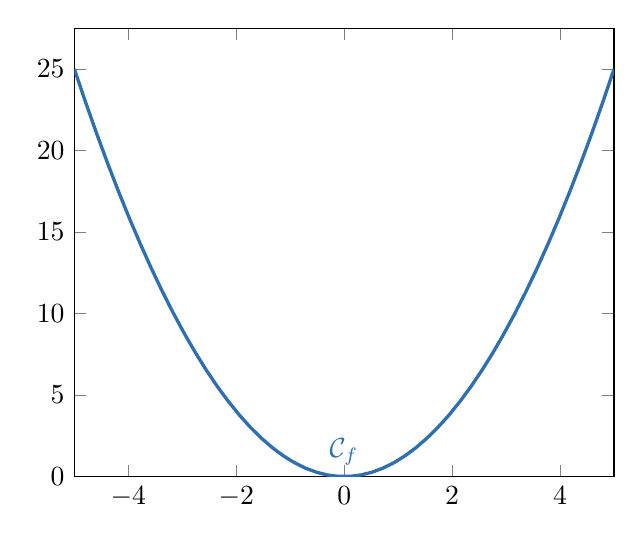
\begin{tikzpicture}
	\begin{axis}[ymin=0, xmin=-5, xmax=5]
		\addplot[very thick, myb, domain=-5:5, samples=50] {x^2} node[pos=.5, above] {$\C_f$};
	\end{axis}
	\end{tikzpicture}
	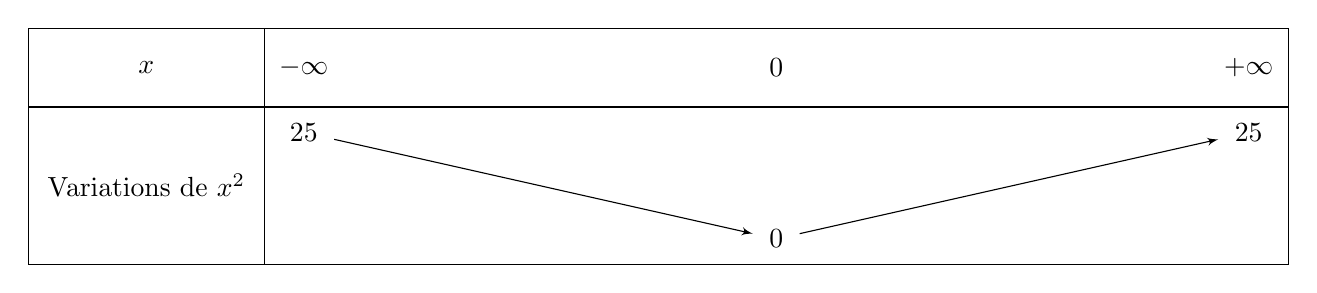
\begin{tikzpicture}
		\tkzTabInit
		 [lgt=3]
	       		{$x$ / 1 , Variations de $x^2$ / 2}
	       		{$\minfty$,, 0 ,,$\pinfty$}
	       		
		
		\tkzTabVar
			{+/25, R/, -/0, R/, +/25}
		
	\end{tikzpicture}
	
	% exe:extrema2
	% page 23
	\begin{tikzpicture}
		\tkzTabInit
		 [lgt=3]
	       		{$x$ / 1 , Variation de $-2x^2$/ 2, Variation de $3x^2$ / 2, Variation de $1+x^2$ / 2, Variation de $2x^2-7$ / 2, Variation de $-3 - 5x^2$ / 2, Variation de $-x^2+17$ / 2}
	       		{,,,,}
	\end{tikzpicture}
	
	% exe:extrema2
	% page 24
	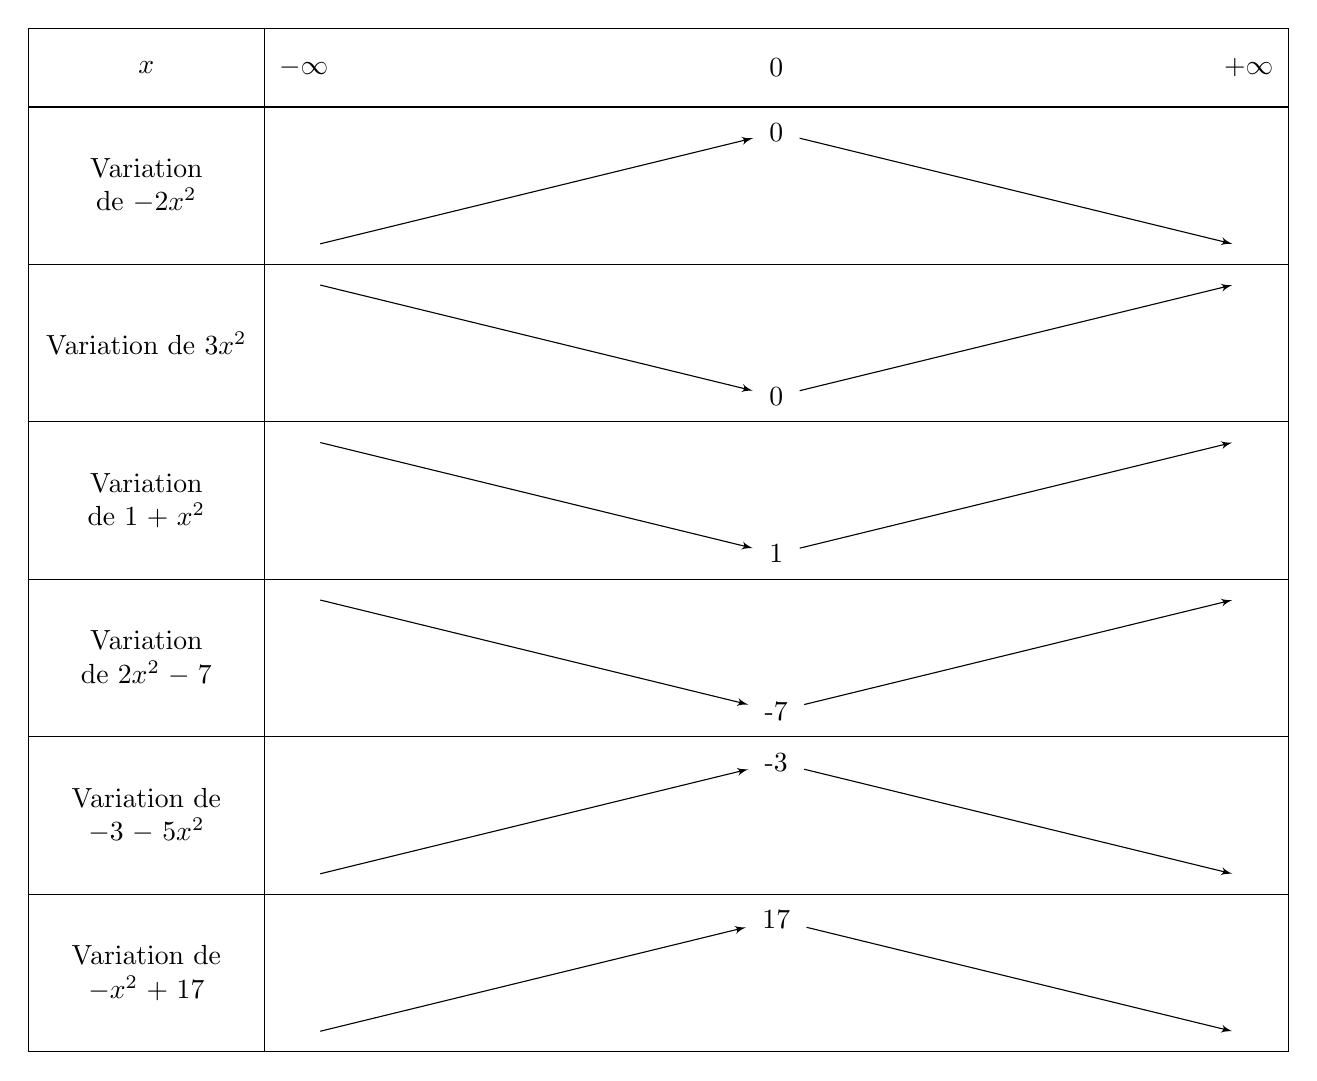
\begin{tikzpicture}
		\tkzTabInit
		 [lgt=3]
	       		{$x$ / 1 , Variation de $-2x^2$/ 2, Variation de $3x^2$ / 2, Variation de $1+x^2$ / 2, Variation de $2x^2-7$ / 2, Variation de $-3 - 5x^2$ / 2, Variation de $-x^2+17$ / 2}
	       		{ $\minfty$ ,, 0 ,,  $\pinfty$ }
	      
		
		\tkzTabVar
			{-/, R/, +/0, R/, -/}
		\tkzTabVar
			{+/, R/, -/0, R/, +/}
		\tkzTabVar
			{+/, R/, -/1, R/, +/}
		\tkzTabVar
			{+/, R/, -/{-7}, R/, +/}
		\tkzTabVar
			{-/, R/, +/{-3}, R/, -/}
		\tkzTabVar
			{-/, R/, +/{17}, R/, -/}
		
	\end{tikzpicture}
	
	% exe:extrema6
	% page 25
	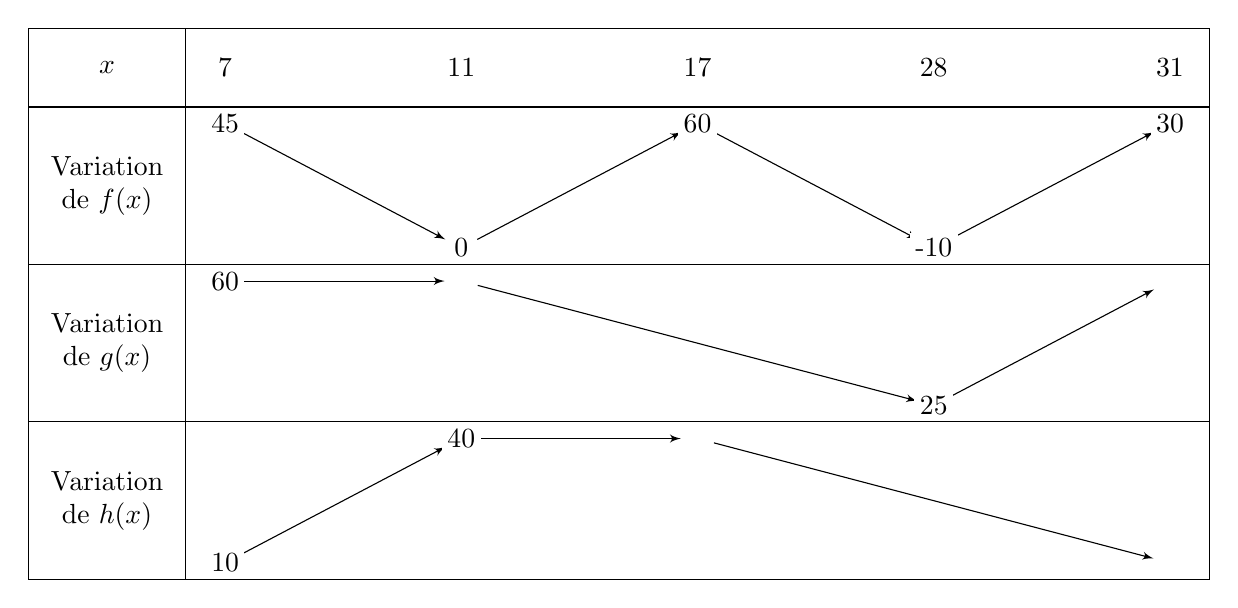
\begin{tikzpicture}
		\tkzTabInit
	       		{$x$ / 1 , Variation de $f(x)$ / 2, Variation de $g(x)$ / 2, Variation de $h(x)$ / 2}
	       		{7,11,17,28,31}

		\tkzTabVar
			{+/,-/,+/,-/,+/}
		\tkzTabIma
			{1}{2}{1}{45}
		\tkzTabIma
			{1}{2}{2}{0}
		\tkzTabIma
			{3}{4}{3}{60}
		\tkzTabIma
			{3}{4}{4}{-10}
		\tkzTabIma
			{4}{5}{5}{30}
			
		\tkzTabVar
			{+/, +/,R/,-/,+/}
		\tkzTabIma
			{1}{2}{1}{60}
		\tkzTabIma
			{2}{4}{4}{25}
			
		\tkzTabVar
			{-/,+/,+/,R/,-/}
		\tkzTabIma
			{1}{2}{1}{10}
		\tkzTabIma
			{1}{2}{2}{40}
	\end{tikzpicture}
	
	% exe:extrema7
	% page 26
	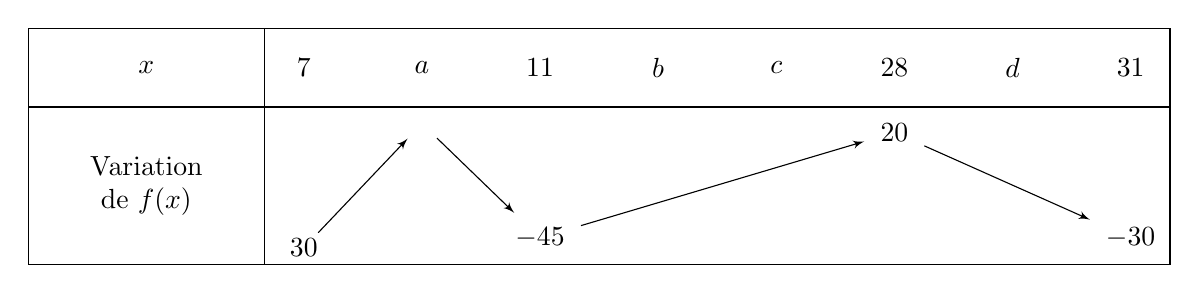
\begin{tikzpicture}
		\tkzTabInit
		 [lgt=3,espcl=1.5]
	       		{$x$ / 1 , Variation de $f(x)$ / 2}
	       		{7,$a$,11,$b$,$c$,28,$d$,31}
			
		\tkzTabVar
			{-/, +/,-/$-45$,R/,R/,+/$20$, R/, -/$-30$}
		\tkzTabIma
			{1}{2}{1}{$30$}
			
	\end{tikzpicture}
%
\end{document}